\documentclass{article}
\usepackage{amsmath}
\usepackage{graphicx}
\usepackage{algorithmic}
\usepackage{algorithm}
\usepackage{color}

\begin{document}
\title{Documentation for Autolab-plot}
\author{Fei Zhan \\ School of Computing Science \\ Simon Fraser University, BC, Canada \\ fzhan@sfu.ca}
\maketitle

\section{Introduction}
A website to demonstrate the figures and trajectories of different robots in Autonomy Lab at Simon Fraser University.
It has been rewritten into libraries in order to facilitate extension.
It is written in HTML, Javascript, PHP, and a little of C++.

\section{framework}
The framework is as Figure \ref{hier}.
I split the plot library and the method library apart in order to avoid large computation on webpage.
The plot library is in charge of generating plots on a webpage, and the method library is for computation on a server.

\begin{figure}
\centering
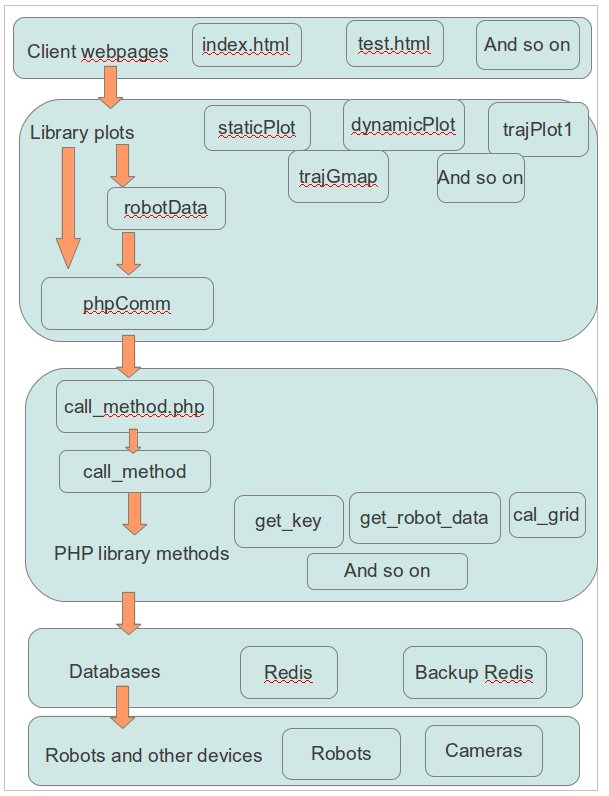
\includegraphics[width=0.8\textwidth]{diagram.jpg}
\caption{Hierarchical chart}
\label{hier}
\end{figure}

\subsection{Client Webpage Level}
Client webpages demonstrate plots with javascript plot libraries.
It can be written in HTML and Javascript by users of Autolab-plot.
When a canvas is reserved in the layout of HTML, an object of a plot class is instantiated, and show function is called, a plot is generated.

In the directory, index.html and test.html belong to this level.

\subsection{Plot Library Level}
Plot Library is utilized to generate various of plots and functional modules of Autolab-plot.
It is called by client webpages.
phpComm is used to communicate with php program, and retrieve data from the server.
The library is written in Javascript as a js file.

Lets take ``staticPlot'' class in plot\_methods.js as an example.
First, create a new HTML file.
To include the library, add the following code into $<head></head>$.

$<script language="javascript" type="text/javascript" src="./flot/jquery.js"></script>$

$<script language="javascript" type="text/javascript" src="./flot/jquery.flot.js"></script>$

$<script src="plot\_methods.js"></script>$

To reserve space for this plot, add the following code into $<body></body>$.

$<div id="staticPlot"></div>$

To create a new static plot, add the following code into $<script></script>$.

var sp = new staticPlot();

To show the plot on a webpage, add

sp.show();

Now, you can see the plot on this webpage.

\subsection{Method Library Level}
The method library is utilized to connect with databases and do some computation on the server.
It is written in PHP, and called by plot library level.
call\_method.php is called directly by a plot library object, and it calls call_method function in connect\_redis.php to assign the corresponding method to call.

Lets take get\_robot\_data function as an example.


\section{Installation}
Autolab-plot is developed in Ubuntu 11.
Compatibility with other platforms is not tested.

Install Apache and PHP first.
Put the entire directory of Autolab-plot into the base directory for the web documents (default as /var/www).
Open a browser and lead to the corresponding url (default as localhost/autolab-plot).
You can see a variety of plots there.

If you want to connect with database and communicate with robots, please install Redis and configure the IP address of Autolab-plot.

\section{Files}
\subsection{connect\_redis.php}
It contains all the service functions that can be called by javascript

\subsection{call\_method.php}
It is called by javascript programs, and calls "call\_method" method in order to parse the "method" parameter and call the corresponding function in PHP.

\section{License}
This program is free software; you can redistribute it and/or modify it under the terms of the GNU General Public License version 3 as published by the Free Software Foundation.

This program is distributed in the hope that it will be useful, but WITHOUT ANY WARRANTY; without even the implied warranty of MERCHANTABILITY or FITNESS FOR A PARTICULAR PURPOSE. See the GNU General Public License for more details.

A copy of the license is included with the sourcecode in the file 'COPYING". Copying and redistribution is permitted only under the terms of the license.

\bibliographystyle{plain}
\bibliography{sample}
\end{document}
